\documentclass{article}

\usepackage[utf8]{inputenc}
\usepackage[ngerman]{babel} 
\usepackage{fancyhdr}
\usepackage{tabularx}
\usepackage{graphicx}
\usepackage{lastpage}
\usepackage{ltablex}
\usepackage{lipsum}
%\usepackage{lscape} % ohne Ändern der Seite
\usepackage{pdflscape} % mit Ändern der Seite
\usepackage{colortbl}

\definecolor{red}{RGB}{255,0,0}
\definecolor{orange}{RGB}{255,165,0}
\definecolor{yellow}{RGB}{255,255,0}
\definecolor{green}{RGB}{0,255,0}


\newcolumntype{L}[1]{>{\raggedright\arraybackslash}p{#1}}
\newcolumntype{C}[1]{>{\centering\arraybackslash}p{#1}}
\newcolumntype{R}[1]{>{\raggedleft\arraybackslash}p{#1}}

\usepackage[
%showframe,% Seitenlayout anzeigen
left=3cm,
right=2cm,
top=2.5cm,
bottom=2cm,
%includeheadfoot
]{geometry}

\pagenumbering{arabic}


\begin{document}
\title{%
	Fallstudie Home-Computer \\
	\large Information Security Fundamentals \\
	Hochschule Luzern}

\author{Florian Bär}
\maketitle
\thispagestyle{empty}
\clearpage
\setcounter{page}{1}

\tableofcontents

\section{Einführung zum Minicase}

Die Familie Meier wohnt in einem dreistöckigen Haus im zweiten Stockwerk. Insgesamt teilen 6 Wohnungen das Haus auf. Eine fortschrittliche Familie aus dem Mittelstand mit bester Reputation.
Bei der Familie Meier wird die IT-Infrastruktur von Onkel Smirnow betreut, welcher von Zeit zu Zeit mit Cracks und anderen Tools das Leben der Familie Meier vereinfacht.


Es folgt der Netzwerkaufbau der Familie Meier zur Veranschaulichung.


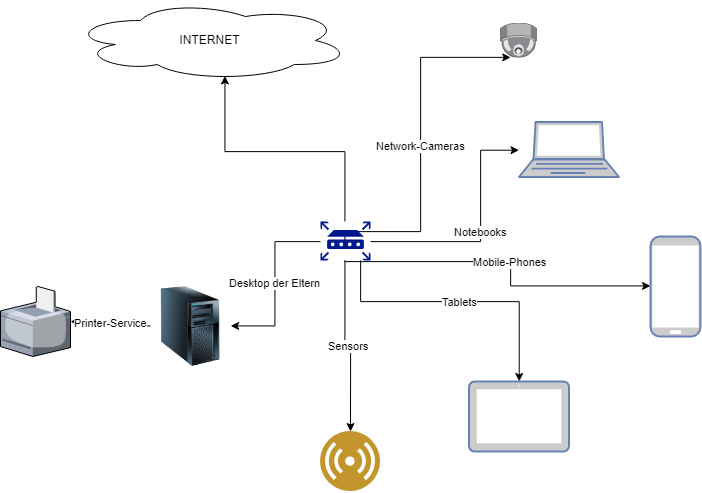
\includegraphics[width=14cm]{./Netzwerk.png}

Für diese Familie sollte ein Massnahmenplan für allfällige Risiken gemäss der Aufgabenstellung \grqq Fallstudie: Die Heim PC Lösung\grqq \space erstellt werden. Für die Eintrittswahrscheinlichkeit und den potenziellen Schaden (Schadensausmass) der Ereignisse wird eine Skala von 1 (sehr kleine(r) Wahrscheinlichkeit/Schaden) bis 4 (sehr grosse(r) Wahrscheinlichkeit/Schaden) verwendet.



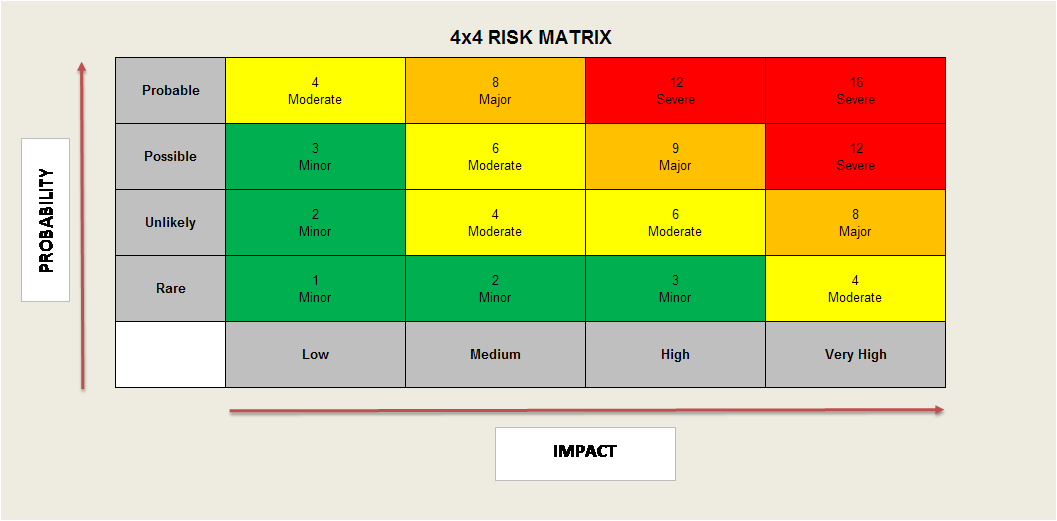
\includegraphics[width=\textwidth]{./Risikomatrix.png}


\newpage


\section{Fallstudie ISF}

\subsection{Risiken}

\subsubsection{Beschreibung der Risiken}

Es folgt eine Liste mit Dingen, welche Sicherheitsrisiken beinhalten:
\begin{enumerate}
\item Das Wireless brauch WEP. WEP ist veraltet und nicht sicher. Es ist ein upgrade
zu WPA2 empfohlen.
\item Die Spiele und Tools, welche Onkel Özutück mitbringt, könnten gecrackt sein.
Cracks beinhalten ein Sicherheitsrisiko. Selbst wenn Sie nicht gefährlich sind, dann
sind diese illegal verwendet.
\item Da Jan ein Computerfreak ist, versucht er bestimmt immer neue Dinge. Dabei wird das Sicherheitsrisiko von diesen “Nerd”-Tools oftmals unterschätzt.
\item Dora ist mit 12 Jahren ein junges Kind. Vor allem bei jungen Kindern sollte der
Internetkonsum kontrolliert werden. Dazu gibt es passende Kinderschutzsoftware.
\item Die Computer müssten auf einem NAS oder einem sonstigen Server ein Backup
haben. Falls einmal eine HD kaputt gehen sollte, sind die Daten nicht wiederherstellbar.
\item Die Kameras könnten von einem Billighersteller sein, welcher die Sicherheitsysteme
des Systems nicht sehr verantwortungsvoll implementiert. Diese könnten dann
“gehackt” werden und einen grossen Eingriff in die Privatsphäre der Familie.
\item Der Desktop PC der Eltern sollte nicht gleichzeitig als PC und als Printserver
verwendet werden. Server öffnen normalerweise Ports und Services für das Netzwerk
und können so ein Sicherheitsrisiko darstellen.
\item Windows Betriebssysteme besitzen zwar den Bitlocker, jedoch ist dieser Standard-
mässig nicht eingeschaltet und kann auch nur von forgeschrittenen Usern bedient
werden. Dadurch sind die Daten auf den Disks nicht verschlüsselt und können unter
Umständen ausgelesen werden.
\item Bei einem Brand wären alle Computer zerstört und es könnten keine Daten wieder-
hergestellt werden.
\item Benutzen die Kinder und die Eltern die selbe Mail? Dies könnte allenfalls auch zu
einem Risiko werden. Nicht alle Mails sind für die Augen der Kinder gedacht.
\end{enumerate}
\newpage

\begin{landscape}

\subsubsection{Risikomatrix}
\begin{tabularx}{\columnwidth}{|r|c|X|c|X|c|}
	\hline
	\textbf{ID} & \textbf{EW\footnote{Eintrittswahrscheinlichkeit}} & \textbf{Begründung} & \textbf{SG\footnote{Schadensgrösse}} & \textbf{Begründung} & \textbf{Risiko} \\ 
	\hline		
	1 &  \cellcolor{red}4 & Da WEP schon veraltet ist und in wenigen Sekunden mit einem mittelklassigen Computer geknackt werden kann ist die Eintrittswahrscheinlichkeit hoch. & \cellcolor{red}4 & Mit Zugriff auf das Netzwerk ist dem “Hacker” alles Möglich	(Zugriff auf Computer, Kameras etc.).  & \cellcolor{red}16 \\ \hline
	2 &  \cellcolor{red}4 & Sehr hoch, da im Text steht, dass der Onkel Özukück gratis Software mitbringt.  & \cellcolor{red}4 & Da Cracks häufig infiziert sind, ist das Risiko für das infizieren mit einer Schadsoftware sehr gross.  & \cellcolor{red}16 \\ \hline
	3 &  \cellcolor{orange}3 &  Es gibt auch auf Github und anderen Clouddiensten viele Schadsoftware, welche als kleine Tools getarnt sind.  & \cellcolor{red}4 & Wenn der PC mit Schadsoftware infiziert wurde, dann ist dieser Computer dieser ausgeliefert.  & \cellcolor{red}12 \\ \hline
	4 &  \cellcolor{red}4 & Da Kinder tendenziell sich am PC explorativ verhalten, kann Dora einfach auf zwilichtige Webseiten gelangen.  & \cellcolor{red}4 & Der Besuch von "schlechten" Webseiten kann die Zukunft von Dora massiv beeinflussen und im schlimmsten Fall dazu führen, dass sie einmal im Gefängnis landet. & \cellcolor{red}16 \\ \hline
	5 &  \cellcolor{orange}3 & Es kann immer einmal ein Laptop auf den Boden fallen. Falls dann eine HD kaputt geht, sind allenfalls gespeicherte Fotos auf diesem Computer verloren. Auch von einer allfälligen Fehlproduktion ist man nicht geschützt. & \cellcolor{orange}3 & Der materielle Schaden ist bei der Familie nicht sehr gross. Allerdings kann der Verlust von Familienfotos sehr schmerzhaft sein. & \cellcolor{orange}9 \\ \hline
	6 &  \cellcolor{yellow}2 & Auch Billigkamerahersteller bemüht, das Sicherheit einem Minimalstandard entspricht. & \cellcolor{orange}3 & Das Interesse von einem Hacker, sich Zugriff auf eine Kamera zu verschaffen ist allerhöchstens von perversem Interesse. & \cellcolor{yellow}6 \\ \hline\textsl{}
	7 &  \cellcolor{yellow}2 & Games und Server öffnen Services für die Multiplayerfähigkeit. Diese stellen potenziell ein Sicherheitsrisiko dar. & \cellcolor{red}4 & Wenn man mit einem Bufferoverflow oder anderen Code-Injection sich Zugriff auf einen PC erschleichen kann, dann ist man Herr über dieses Gerät. & \cellcolor{orange}8 \\ \hline
	8 &  \cellcolor{yellow}2 & Damit man an die Daten des Computers kommt, muss man zuerst Zugriff auf diesen Computer haben. Dies ist nur bei einem Einbruch oder einem Diebstahl möglich. & \cellcolor{orange}3 & Wenn man allerdings einmal Zugriff auf diesen Computer hat, dann ist es einer Fremdperson möglich, alle Daten\footnote{inkl. Passwörter und persönliche Unterlagen} auszulesen.  & \cellcolor{yellow}6 \\ \hline
	9 &  \cellcolor{yellow}2 & Dass alle Daten und Backups zerstört werden ist grundsätzlich nur bei einem Brand möglich. Diese sind in der Schweiz zum Glück selten. & \cellcolor{red}4 & Wenn ein Brand ausbrechen würde, dann wären alle Daten und auch deren (allenfalls gemachten) Back-Ups zerstört. & \cellcolor{orange}8 \\ \hline
	10 &  \cellcolor{orange}3 & Normalerweise interessieren sich die Kinder nicht für die Mails der Eltern. Und um Schaden zu verursachen, müsste dies Mutwillig seitens der Kinder geschehen. & \cellcolor{yellow}2 & Die Eltern haben normalerweise nicht viele (bis keine) Information, welche Schaden anrichten können. & \cellcolor{yellow}6 \\ \hline
\end{tabularx}

\newpage

\end{landscape}

\begin{landscape}


\include{Risikomatrix}


\subsection{Massnahmen}

\subsubsection{Beschreibung der Massnahmen}

1. WEP mit WPA2 ersetzen
• Auf dem Router anstelle von WEP ein WPA2 Passwort setzen. WPA2 ist
viel schwerer zu intercepten und somit besteht ein geringers Risiko von einem
unerwünschten Zugriff.
• Eintrittswahrscheinlichkeit: 1
• Schaden: 2
2. Teuererer Router mit Guest-Netz Funktion kaufen (z.B. Router ASUS RT-AC88U)
• Somit ist es Gästen der Familie Meier nicht mehr möglich auf die selben
Home-Resourcen zuzugreifen.
• Eintrittswahrscheinlichkeit: 2
• Schaden: 1
3. Arbeits-PC von Spiele PC trennen.
• Spiele können ungewollt Ports eines Systemes öffnen und damit ein Risiko
darstellen. Zudem könne Mods (von Sohn Jan installiert) Sicherheitslücken
beinhalten und ein Problem darstellen. Nach dieser Trennung sind grössere
Lücken beim Arbeits-PC geschlossen.
• Eintrittswahrscheinlichkeit: 2
• Schaden: 2
4. Dora nur ein Laptop mit “Kindersicherung” geben. Dazu Dora keine Administra-
torenrechte geben. Diese Rechte reichen dem Kind.
• Dora kann nun keine unerwünschte Software mehr installieren und von Ihr
geht somit keine Gefahr mehr aus.
• Eintrittswahrscheinlichkeit: 1
• Schaden: 2
5. NAS kaufen, um ein Backup von Daten zu machen. Dieses NAS könnte auch
mittels Docker einen PrinterServer hosten, was auch das Problem der geöffneten
Ports des Arbeits-PCs löst.
• Daten sind nun Zentral gesichert. Bei einem allfälligen Hardware-Defekt sind
die Daten nicht verloren.
• + Option auf Google Business-Account um Backup verschlüsselt auf die Cloud
zu synchronisieren
• Eintrittswahrscheinlichkeit: 1
• Schaden: 3
6. Einen zweiten Router kaufen, um die Sensoren und Kameras in ein anderes Netz
zu stellen.
• Durch diese Netztrennung, ist das Heimnetz von allfälligen Hackerangriffen
besser geschützt.
• Eintrittswahrscheinlichkeit: 1
• Schaden: 3
7. Alle Computer mit Passwort sichern. Es sollten auf die Computer jeweils nur die
Familienmitglieder Zugriff haben, welche dazu auch befugt sind.
• Der Zugriff auf die Computer bei einem Diebstahl ist erschwert und die Daten
auf diesen Computern sind besser geschützt.
• Eintrittswahrscheinlichkeit: 1
• Schaden: 1
8. Software von Onkel Özutück sollte über den offiziellen Weg gekauft werden.
• Die installierte Software ist sicher legal gekauft und hat mit einer grossen
Wahrscheinlichkeit keine grossen Sicherheitsrisiken.
• In betracht ziehen, dass Onkel Özutück in Zukunft die Computer nicht mehr
verwalten sollte.
• Eintrittswahrscheinlichkeit: 2
• Schaden: 1
9. Für die Arbeiten, welche Herr Meier zu Hause macht sollte ein Arbeits-PC mit
nach Hause genommen werden können. Diese sind in der Regel von der zuständigen
IT-Abteilung genügen sicher “gehardened”.
• Die Familie muss sich nicht um die Sicherheit der Arbeitsdaten von Herrn
Meier kümmern.

• Eintrittswahrscheinlichkeit: 0
• Schaden: 1
10. Auch auf Smartphones und Tablets Antivirenprogramme installieren. Auch wenn
diese noch nicht sehr verbreitet sind, besteht durch Schadsoftware an Handys bereits
heute ein beträchtlicher Schaden.
• AdWare und andere Schadsoftware wird auf dem Smartphone und Tablet
erkannt. Somit sind nicht nur die Daten besser gschützt.
• Eintrittswahrscheinlichkeit: 2
• Schaden: 1

\begin{landscape}
\newpage
\subsubsection{Risikomatrix nach Massnahmen}

\begin{tabular}{|R{1cm}|C{4cm}|C{6.5cm}|C{2cm}|C{6.5cm}|C{2cm}|}
	\hline
	ID & Eintrittswahrscheinlichkeit & Begründung & Schadensgrösse & Begründung & Risiko \\ \hline
	1 &  \cellcolor{red}4 & GRUND & \cellcolor{red}4 & GRUND  & \cellcolor{red}16 \\ \hline
	2 &  \cellcolor{red}4 & GRUND  & \cellcolor{red}4 & GRUND  & \cellcolor{red}16 \\ \hline
	3 &  \cellcolor{orange}3 & GRUND  & \cellcolor{green}4 & GRUND  & \cellcolor{yellow}12 \\ \hline
	4 &  \cellcolor{red}4 & GRUND  & \cellcolor{red}4 & GRUND  & \cellcolor{red}16 \\ \hline
	5 &  \cellcolor{orange}3 & GRUND  & \cellcolor{orange}3 & GRUND  & \cellcolor{red}9 \\ \hline
	6 &  \cellcolor{yellow}2 & GRUND  & \cellcolor{orange}3 & GRUND  & \cellcolor{red}6 \\ \hline
	7 &  \cellcolor{yellow}2 & GRUND  & \cellcolor{orange}3 & GRUND  & \cellcolor{red}6 \\ \hline
	8 &  \cellcolor{yellow}2 & GRUND  & \cellcolor{orange}3 & GRUND  & \cellcolor{red}6 \\ \hline
	9 &  \cellcolor{yellow}2 & GRUND  & \cellcolor{red}4 & GRUND  & \cellcolor{red}8 \\ \hline
	10 &  \cellcolor{orange}3 & GRUND  & \cellcolor{yellow}2 & GRUND  & \cellcolor{red}6 \\ \hline
\end{tabular}


\newpage
\end{landscape}
\section{Fazit}



\end{document}
